\documentclass[12pt,letterpaper]{report}
\usepackage[square,numbers]{natbib}
\usepackage{geometry}
\usepackage{fancyhdr}
\usepackage{afterpage}
\usepackage{graphicx}
\usepackage{amsmath,amssymb,amsbsy}
\usepackage{dcolumn,array}
\usepackage{tocloft}

% for title case
\usepackage{titlecaps}
\Addlcwords{and, the, or, of, that, our, by}

% avoid widows
\usepackage[all]{nowidow}
\clubpenalty=10000

\usepackage{asudis}
%% These are for including code
%% and for upquotes
\usepackage[T1]{fontenc}
\usepackage{textcomp}
\usepackage{listings}
\usepackage{listingsutf8}
\usepackage{comment}
\usepackage{color}
\usepackage{dirtytalk} % for quotations
\usepackage[justification=centering]{caption}
\usepackage[pageanchor=true,plainpages=false,pdfpagelabels,bookmarks,bookmarksnumbered,hidelinks]{hyperref}


% for footnotes in tables
\usepackage{tablefootnote}

% for arithmetic
\usepackage{xintexpr}

\usepackage{textcomp}     % access \textquotesingle

\definecolor{mygray}{rgb}{0.6,0.6,0.6}
\definecolor{lightgray}{rgb}{0.92,0.92,0.92}
\definecolor{darkgreen}{rgb}{0,0.7,0}
% default options for listings
\lstset{
	backgroundcolor=\color{lightgray},
	basicstyle=\footnotesize,
	breaklines=true, 
	captionpos=b,
	commentstyle=\color{darkgreen}, 
	frame=single,
	keywordstyle=\color{blue}, 
	numbers=left,
	numbersep=5pt,
	numberstyle=\tiny\color{mygray},
	rulecolor=\color{black},
	showstringspaces=false,
	upquote=true
}

	
\newcommand{\dq}[1]{``{#1}''}
%% THIS IS THE DATA FOR OUR THESIS, UPDATING HERE WILL UPDATE EVERYWHERE %%
\newcommand{\urls}{17,686,161}

\newcommand{\forms}{5,562,533}
\newcommand{\formsDelta}{31.45\%}

\newcommand{\emailforms}{918,988}
\newcommand{\emailformsDelta}{16.52\%}

\newcommand{\fuzzed}{756,588}
\newcommand{\fuzzedDelta}{82.33\%}

\newcommand{\recd}{44,735}
\newcommand{\recdDelta}{5.91\%}

\newcommand{\malfuzzed}{38,989}
\newcommand{\malfuzzedDelta}{87.16\%}

\newcommand{\success}{433}
\newcommand{\successDelta}{1.11\%}

\newcommand{\domains}{182}

% these refer to unique domains, not unique forms
\newcommand{\uniqueforms}{650,394}
\newcommand{\uniqueemailforms}{151,795}

\begin{document}
%-----------------------front matter
\pagenumbering{roman}
\title{E-Mail Header Injections\\
	An Analysis of the World Wide Web}

\author{Sai Prashanth Chandramouli}
\degreeName{Master of Science}
\paperType{Thesis}
\defensemonth{April}
\defenseyear{2016}
\gradmonth{May}
\gradyear{2016}
\chair{Adam Doup\'{e}}
\memberOne{Gail-Joon Ahn}
\memberTwo{Ziming Zhao}
%%\memberThree{Your third member}
%%\memberFour{Your third member}

\maketitle
\doublespace
\begin{abstract}
	E-mail header injection vulnerability is a class of vulnerability that has been around for a long time but has not made its way to popular literature. It can be considered as the e-mail equivalent of HTTP Header Injection Vulnerability. Email injection is possible when the mailing script fails to check for the presence of e-mail headers in the form fields that take in e-mail addresses. The vulnerability exists in the reference implementation of the built-in “mail” functionality in popular languages like PHP, Java, Python, and Ruby\@. With the proper injection string, this vulnerability can be exploited to inject additional headers and/or modify existing headers in an E-mail message.
	\paragraph{}
	This thesis serves to understand and quantify the prevalence of E-Mail Header Injection vulnerabilities. Using a black-box testing approach, we crawled \urls\ URLs in order to find the URLs which contained form fields. We found \forms\ such forms, out of which \emailforms\ forms contained e-mail fields. Our system used this data feed to classify which of these forms could be fuzzed with malicious payloads. Amongst the \fuzzed\ forms tested, \recd\ forms were found to be fuzzable. Our system tested \malfuzzed\ of these, and was able to find \success\ vulnerable URLs across \domains\ domains, which proves that the threat is widespread and deserves future research attention.

\end{abstract}

\dedicationpage{To my mother and father, for giving me the life I dreamt of,\\
To my sister, who constantly made me do better just to keep up with her,\\
To my family in Phoenix, for always being there,\\
To God, for making me so lucky, for letting me be strong when I had nothing, and making me believe when no one else would have.}
\begin{acknowledgements}
	A project of this size is never easy to complete without the help and support of other people. I would like to take this opportunity to thank some of them.

This thesis would not have been possible without the help and guidance of my thesis advisor, and committee chair - the brilliant Dr. Adam Doupe.
This project was his brainchild, and he held my hand through the entire project.

I would like to thank Dr. Gail-Joon Ahn, for being part of the committee, for all his help, and his valuable input on the changes to be made to make the project more impactful.

I would also like to thank Dr. Ziming Zhao, for being a part of my committee, and for the constant motivation.

I would like to thank the members of the SEFCOM, for their support, and would like to especially thank Mike Mabey, for helping set up the infrastructure for this project, and Marthony Taguinod, for helping me document this project.
\end{acknowledgements}
\tableofcontents
% This puts the word "Page" right justified above everything else.
\addtocontents{toc}{~\hfill Page\par}
% Asking LaTeX for a new page here guarantees that the LOF is on a separate page
% after the TOC ends.
\newpage
% Making the LOT and LOF "parts" rather than chapters gets them indented at
% level -1 according to the chart: top of page 4 of the document at
% ftp://tug.ctan.org/pub/tex-archive/macros/latex/contrib/tocloft/tocloft.pdf
\addcontentsline{toc}{part}{LIST OF TABLES}
\renewcommand{\cftlabel}{Table}
\listoftables
% This gets the headers for the LOT right on the first page.  Subsequent pages
% are handled by the fancyhdr code in the asudis.sty file.
\addtocontents{lot}{Table~\hfill Page \par}
\newpage
\addcontentsline{toc}{part}{LIST OF FIGURES}
\addtocontents{toc}{CHAPTER \par}
\renewcommand{\cftlabel}{Figure}
% This gets the headers for the LOF right on the first page.  Subsequent pages
% are handled by the fancyhdr code in the asudis.sty file.
\addtocontents{lof}{Figure~\hfill Page \par}
\listoffigures
%-----------------------body
\doublespace
\pagenumbering{arabic}
\chapter{Introduction}
\paragraph{}
	The World Wide Web has single-handedly brought about a change in the way we use computers. The ubiquitous nature of the Web has made it possible for the general public to access it anywhere and on multiple devices like phones, laptops, personal digital assistants, and even on TVs and cars. This has ushered in an era of responsive web applications which depend on user input. While this rapid pace of development has improved the speed of dissemination of information, it does come at a cost. Attackers have an added incentive to break into user's e-mail accounts more than ever. E-Mail accounts are usually connected to almost all other online accounts of a user, and e-mails continue to serve as the principal mode of official communication on the web for most institutions. Thus, the impact an attacker can have by having control over the e-mail communication sent by websites to users is of an enormous magnitude. 
	
	Since attackers typically masquerade themselves as users of the system, if user input is to be trusted, then developers need to have proper sanitization routines in place. Many different injection attacks such as SQL injection or cross-site scripting (XSS) \cite{OWASPT10} are possible due to improper sanitization of user input. 
	
	Our research focuses on a lesser known injection attack known as E-Mail Header Injection. E-Mail Header Injection can be considered as the e-mail equivalent of HTTP Header Injection vulnerability \cite{wiki:HTTP_headerinjection}. The vulnerability exists in the reference implementation of the built-in \dq{\texttt{mail}} functionality in popular languages like PHP, Java, Python, and Ruby. With the proper injection string, this vulnerability can be exploited to inject additional headers and/or modify existing headers in an e-mail message --- with the potential to alter the contents of the e-mail message --- while still appearing to be from a legitimate source.
	
	E-Mail Header Injection attacks have the potential to allow an attacker to perform e-mail spoofing, resulting in phishing attacks that can lead to identity theft.
	The objective of our research is to study the prevalence of this vulnerability on the World Wide Web, and identify whether further research is required in this area.
	
	We performed an expansive crawl of the web, extracting forms with e-mail fields, and injecting them with different payloads to infer the existence of E-mail Header Injection vulnerability. We then audited received e-mails to see if any of the injected data was present. This allowed us to classify whether a particular URL was vulnerable to the attack. The entire system works in a black-box manner, without looking at the web application's source code, and only analyzes the e-mails we receive based on the injected payloads.

\paragraph{Structure of document} % describes the remaining sections and gives a short desc about them
This thesis document is divided logically into the following sections:
\begin{itemize}
	\item Chapter 2 discusses the background of e-mail header injection, a brief history of the vulnerability, and enumerates the languages and platforms affected by this vulnerability.
	
	\item Chapter 3 discusses the System design, the architecture, and the components of the system.
	
	\item Chapter 4 describes the experimental setup and sheds light on how we overcame the issues and assumptions discussed in Chapter 3.
	
	\item Chapter 5 presents our findings and our analysis of the results.
	
	\item Chapter 6 continues the discussion of the results; the lessons learned over the course of the project, limitations, and a suitable mitigation strategy to overcome the vulnerability.
	
	\item Chapter 7 explores related work in the area.
	
	\item Chapter 8 concludes this thesis, with ideas to expand the research in this area.
\end{itemize} 

\paragraph{} % summary paragraph
We hope that our research sheds some light on this relatively less well-known vulnerability, and find out its prevalence on the World Wide Web. In summary, we make the following contributions:
\begin{itemize}
	
	\item{A black-box approach to detecting the presence of E-Mail header injection vulnerability in a web application.}
	
	\item{A detection and classification tool based on the above approach, which will automatically detect such E-Mail Header Injection vulnerabilities in a web application.}
	
	\item{A quantification of the presence of such vulnerabilities on the World Wide Web, based on a crawl of the Web, including \urls\ URLs and \forms\ forms.}
	
\end{itemize}

\paragraph{}
\chapter{E-Mail Header Injection Background}
% need to fix this chapter soon
This chapter goes into the background of the problem at hand and gives a brief history of E-Mail Header Injection. It then describes the languages affected by this vulnerability and discusses the overall impact E-Mail Header Injection can have, and the attacks that can result from this vulnerability.
\section{Problem Background}

E-Mail Header Injection belongs to a broad class of Vulnerabilities known simply as Injection attacks. However, unlike its more popular siblings, SQL injection (\cite{sql0}, \cite{sql1}, \cite{sql2}), cross-site scripting (XSS) (\cite{Injection1} \cite{KleinAmit}) or even HTTP Header Injection (\cite{sessionride}), relatively little research is available on E-Mail Header Injection.

As with other vulnerabilities in this class, E-Mail Header Injection is caused due to improper sanitization (or lack thereof) of user input. If the mailing script fails to check for the presence of E-Mail headers in the form fields that take in user input to send E-Mails, a malicious user, using a well-crafted payload, can control the headers set for this particular E-Mail. Suffice it to say, that this can be leveraged to do a host of malicious attacks, including, but not limited to, spoofing, phishing, etc.
\section{History of E-Mail Injection}

E-Mail Header Injection seems to have been first documented over a decade ago, in a late 2004 Article on phpsecure.info (\cite{Tobozo}) accredited to user tobozo@phpsecure.info describing how this vulnerability existed on the reference implementation of the mail function in PHP, and how it can be exploited. More recently, a blog post by Damon Kohler (\cite{DK}) and an accompanying wiki article (\cite{Injection}) describe the attack vector, and outline a few defense measures for the same.

Since this vulnerability was initially found in the \emph{mail()} function of PHP, E-Mail Header Injection can be traced to as early as early 2000's, present in the \emph{mail()} implementation of PHP 4.0. 

The vulnerability was also described very briefly (less than a page) by Stuttard and Pinto in their widely acclaimed book, ``\emph{The Web Application Hacker's Handbook: Discovering and Exploiting Security Flaw}'' (\cite{stuttard2011web}). 
A concise timeline of the vulnerability is presented in Table \ref{tab:history}.

\begin{table}[!htbp]
	\centering
	\begin{tabular}{|p{2cm}|p{12cm}|}
		\hline
		\multicolumn{1}{|c|}{\textbf{Year}} & \multicolumn{1}{c|}{\textbf{ Notes}}\\
		\hline

		{Early 2000's } & { PHP 4.0 is released, along with support for the mail() function, which has no protection against E-Mail Header Injection.}\\
		\hline

		{Jul 2004} & { Next Major version of PHP - Version 5.0 releases}\\
		\hline

		{Dec 2004} & { First known article about the vulnerability surfaces on phpsecure.info}\\
		\hline

		{Oct 2007} & {The vulnerability makes its way into a text by Stuttard and Pinto. }\\
		\hline

		{Dec 2008} & {Blog post and accompanying wiki about the header injection attack in detail with examples.}\\
		\hline

		{Apr 2009} & {Bug filed about email.header package to fix the issue on Python Bug Tracker}\\
		\hline

		{Jan 2011} & {Bug fix for Python 3.1, Python 3.2, Python 2.7 for email.header package, backport to older versions not available.}\\
		\hline

		{Sep 2011} & {The vulnerability is described with an example in the 2nd edition of the text by Stuttard and Pinto.}\\
		\hline

		{Aug 2013} & {Acunetix adds E-Mail Header Injection to the list of vulnerabilties they detect, as part of their Enterprise Web Vulnerability Scanner Software.}\\
		\hline

		{May 2014} & {Security Advisory for JavaMail SMTP Header Injection via method setSubject is written by Alexandre Herzog.}\\
		\hline

		{Dec 2015}  & {PHP 7 releases, mail function still unpatched.}\\
		\hline
	\end{tabular}
	\caption[\titlecap{A brief history of e-mail header injection}]{A brief history of e-mail header injection.}
	\label{tab:history}
\end{table}


\section{Languages Affected}

This section describes the popular languages which exhibit this type of vulnerability. 
\begin{itemize}
	\item PHP - Describe which functions/params are affected
	\item Java - Describe which functions/params are affected
	\item Python - Describe which functions/params are affected
\end{itemize}
 

\section{Potential Impact}

The impact of the vulnerability can be pretty far-reaching.
Table~\ref{tab:usage} shows the current Server side language usage statistics on the Web, compiled from \cite{W3techs}. 
PHP, Java, Python and Ruby (combined) account for over 85\%\footnote{Note: a website may use more than one server-side programming language} of the websites in existence. The vulnerability can be exploited to do potentially any of the following:


\begin{itemize}
	\item Phishing and Spoofing Attacks\\
    Phishing (a variation of spoofing) refers to an attack where the recipient of an E-Mail is made to believe that the E-Mail is a legitimate one. The E-Mail usually redirects them to a malicious website, which then steals their credentials. 
    
    E-Mail Header Injection gives attackers the ability to inject arbitrary headers into an E-Mail sent by a website and control the output of the E-Mail. This adds credibility to the generated E-Mail, and can result in more successful phishing attacks.
	
	\item Spam Networks\\
	Spam networks can capitalize on the ability to send a large amount of E-Mail from servers that are trusted. By adding additional `cc' or `bcc' headers to the generated E-Mail, attackers can easily achieve this effect. 
	
	Due to the E-Mails being from trusted domains, E-Mail clients might not flag them as `spam'. If they do flag them as `spam', then that can lead to the website getting blacklisted as a spam generator. Irrespective of the behavior of spam filters, this does not bode well for the website.
	
	\item Information Extraction of legitimate users\\
	E-Mails can contains sensitive data that is meant to be accessed only by the user. Due to E-Mail Header Injection, an attacker can easily add a `bcc' header, and send the E-Mail to himself, thereby extracting important information.
	User Privacy can thus be compromised, and loss of private information can by itself lead to a host of other attacks.
	
	\item Denial of service by attacking the underlying mail server\\
    Denial of service attacks (DoS as they are popularly known), can also be aided by E-Mail Header Injection. The ability to send hundreds of thousands of E-Mails by just injecting one header field can result in overloading the mail server, and cause crashes and/or instability.
\end{itemize}

It is evident that if proper validation for E-Mail is not performed by these sites, this can quickly escalate to a huge issue.

\begin{table}[!htbp]
	\centering
	\begin{tabular}{|p{4cm}|p{4cm}|}
		\hline
		\multicolumn{1}{|c|}{\textbf{Server Side Language}} & \multicolumn{1}{c|}{\textbf{\% of Usage}}\\
		\hline
		PHP & 81.9\\
		\hline    
		ASP.NET & 15.8\\
		\hline
		Java & 3.1\\
		\hline
		Ruby & 0.6\\
		\hline
		Perl & 0.5\\
		\hline
		JavaScript & 0.2\\
		\hline
		Python & 0.2\\
		\hline
		
	\end{tabular}
	\caption{Language usage statistics compiled from w3techs \cite{W3techs}.}
	\label{tab:usage}
\end{table}

\chapter{System Design}
\section[Approach]{Our Approach to the Problem}
\label{sys:appr}
We took a black-box approach to find out the prevalence of this vulnerability on the World Wide Web. According to \cite{wiki:Black-box_testing}:
\begin{quote}
	``{Black-box testing is a method of software testing that examines the functionality of an application without peering into its internal structures or workings.}''
\end{quote} 

Since we did not have the source code for each of these websites (and even if we did, the sheer number of websites would have made it a \emph{very} tall task), black-box testing was the ideal approach for this project.
Black-box testing gave us the freedom to not worry about the underlying code for the website under test, letting us concentrate on the payload instead.
\section{System Architecture}
\label{sys:arch}
The black-box testing system can be divided broadly into two modules:
\begin{enumerate}
	\item Data Gathering\\
		The Data Gathering module (shown in Fig. \ref{fig:crawler}) is primarily responsible for the following activities:
		\begin{itemize}
			\item Interface with the UCSB Crawler (Section \ref{Comp:Crawler}) and receive the URLs.
			\item Parse the HTML for the corresponding URL, and store the relevant form data (Section \ref{Comp:FP}).
			\item Check for the presence of forms that allow the user to send/receive E-Mail, and store references to these forms (Section \ref{Comp:EMFC}).
		\end{itemize} 
	\item Payload Injection\\
		The Payload Injection module (shown in Fig. \ref{fig:fuzzer}) is primarily responsible for the following activities:
		\begin{itemize}
			\item Retrieve the forms that allow users of a website to send/receive E-Mail, and reconstruct these forms (Section \ref{Comp:EMFR}).
			\item Inject these forms with benign data (non-malicious payloads), generate a HTTP request to the corresponding URL (Section \ref{Comp:Fuzzer:nmp}).
			\item Analyze the E-Mails, extracting the header fields, and checking for the presence of the injected payloads (Section \ref{Comp:EMA}).
			\item Inject the forms that sent us E-Mails with malicious payloads, generate a HTTP request to the corresponding URL to check if E-Mail Header Injection vulnerability exists in that form (Section \ref{Comp:Fuzzer:mp}).
		\end{itemize} 
	The functionality of each component is discussed further in the `Components' section (\ref{Comp}). It is to be noted that the Payload Injection pipeline is not linear, but is a cyclic process.
\end{enumerate}

\begin{figure}
     \centering
     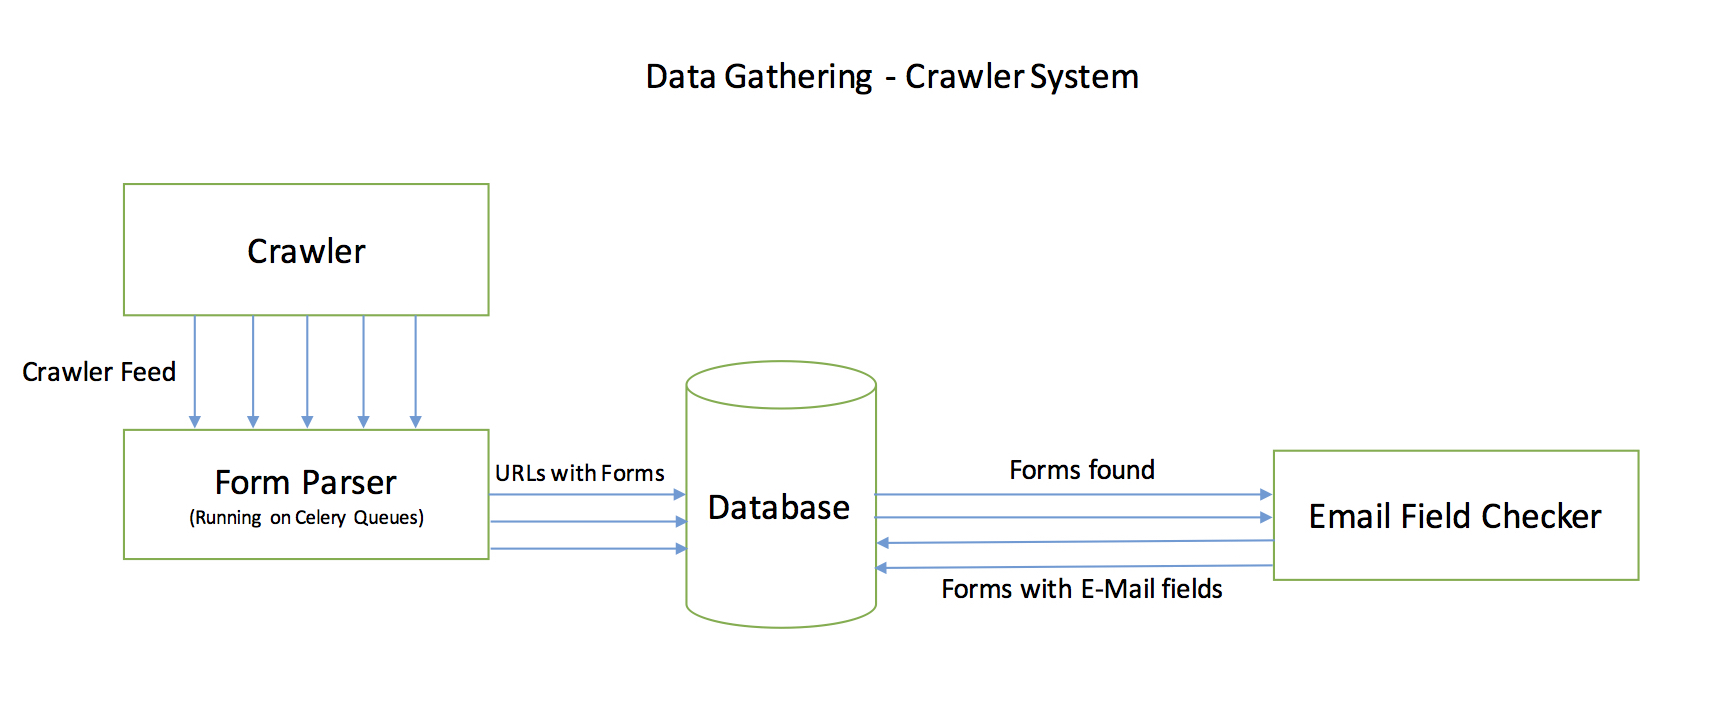
\includegraphics[width=16cm, height=7cm]{System/crawler_design}
     \caption{System Architecture - Crawler}
     \label{fig:crawler}
 \end{figure}
 
 
 \begin{figure}
 	\centering
 	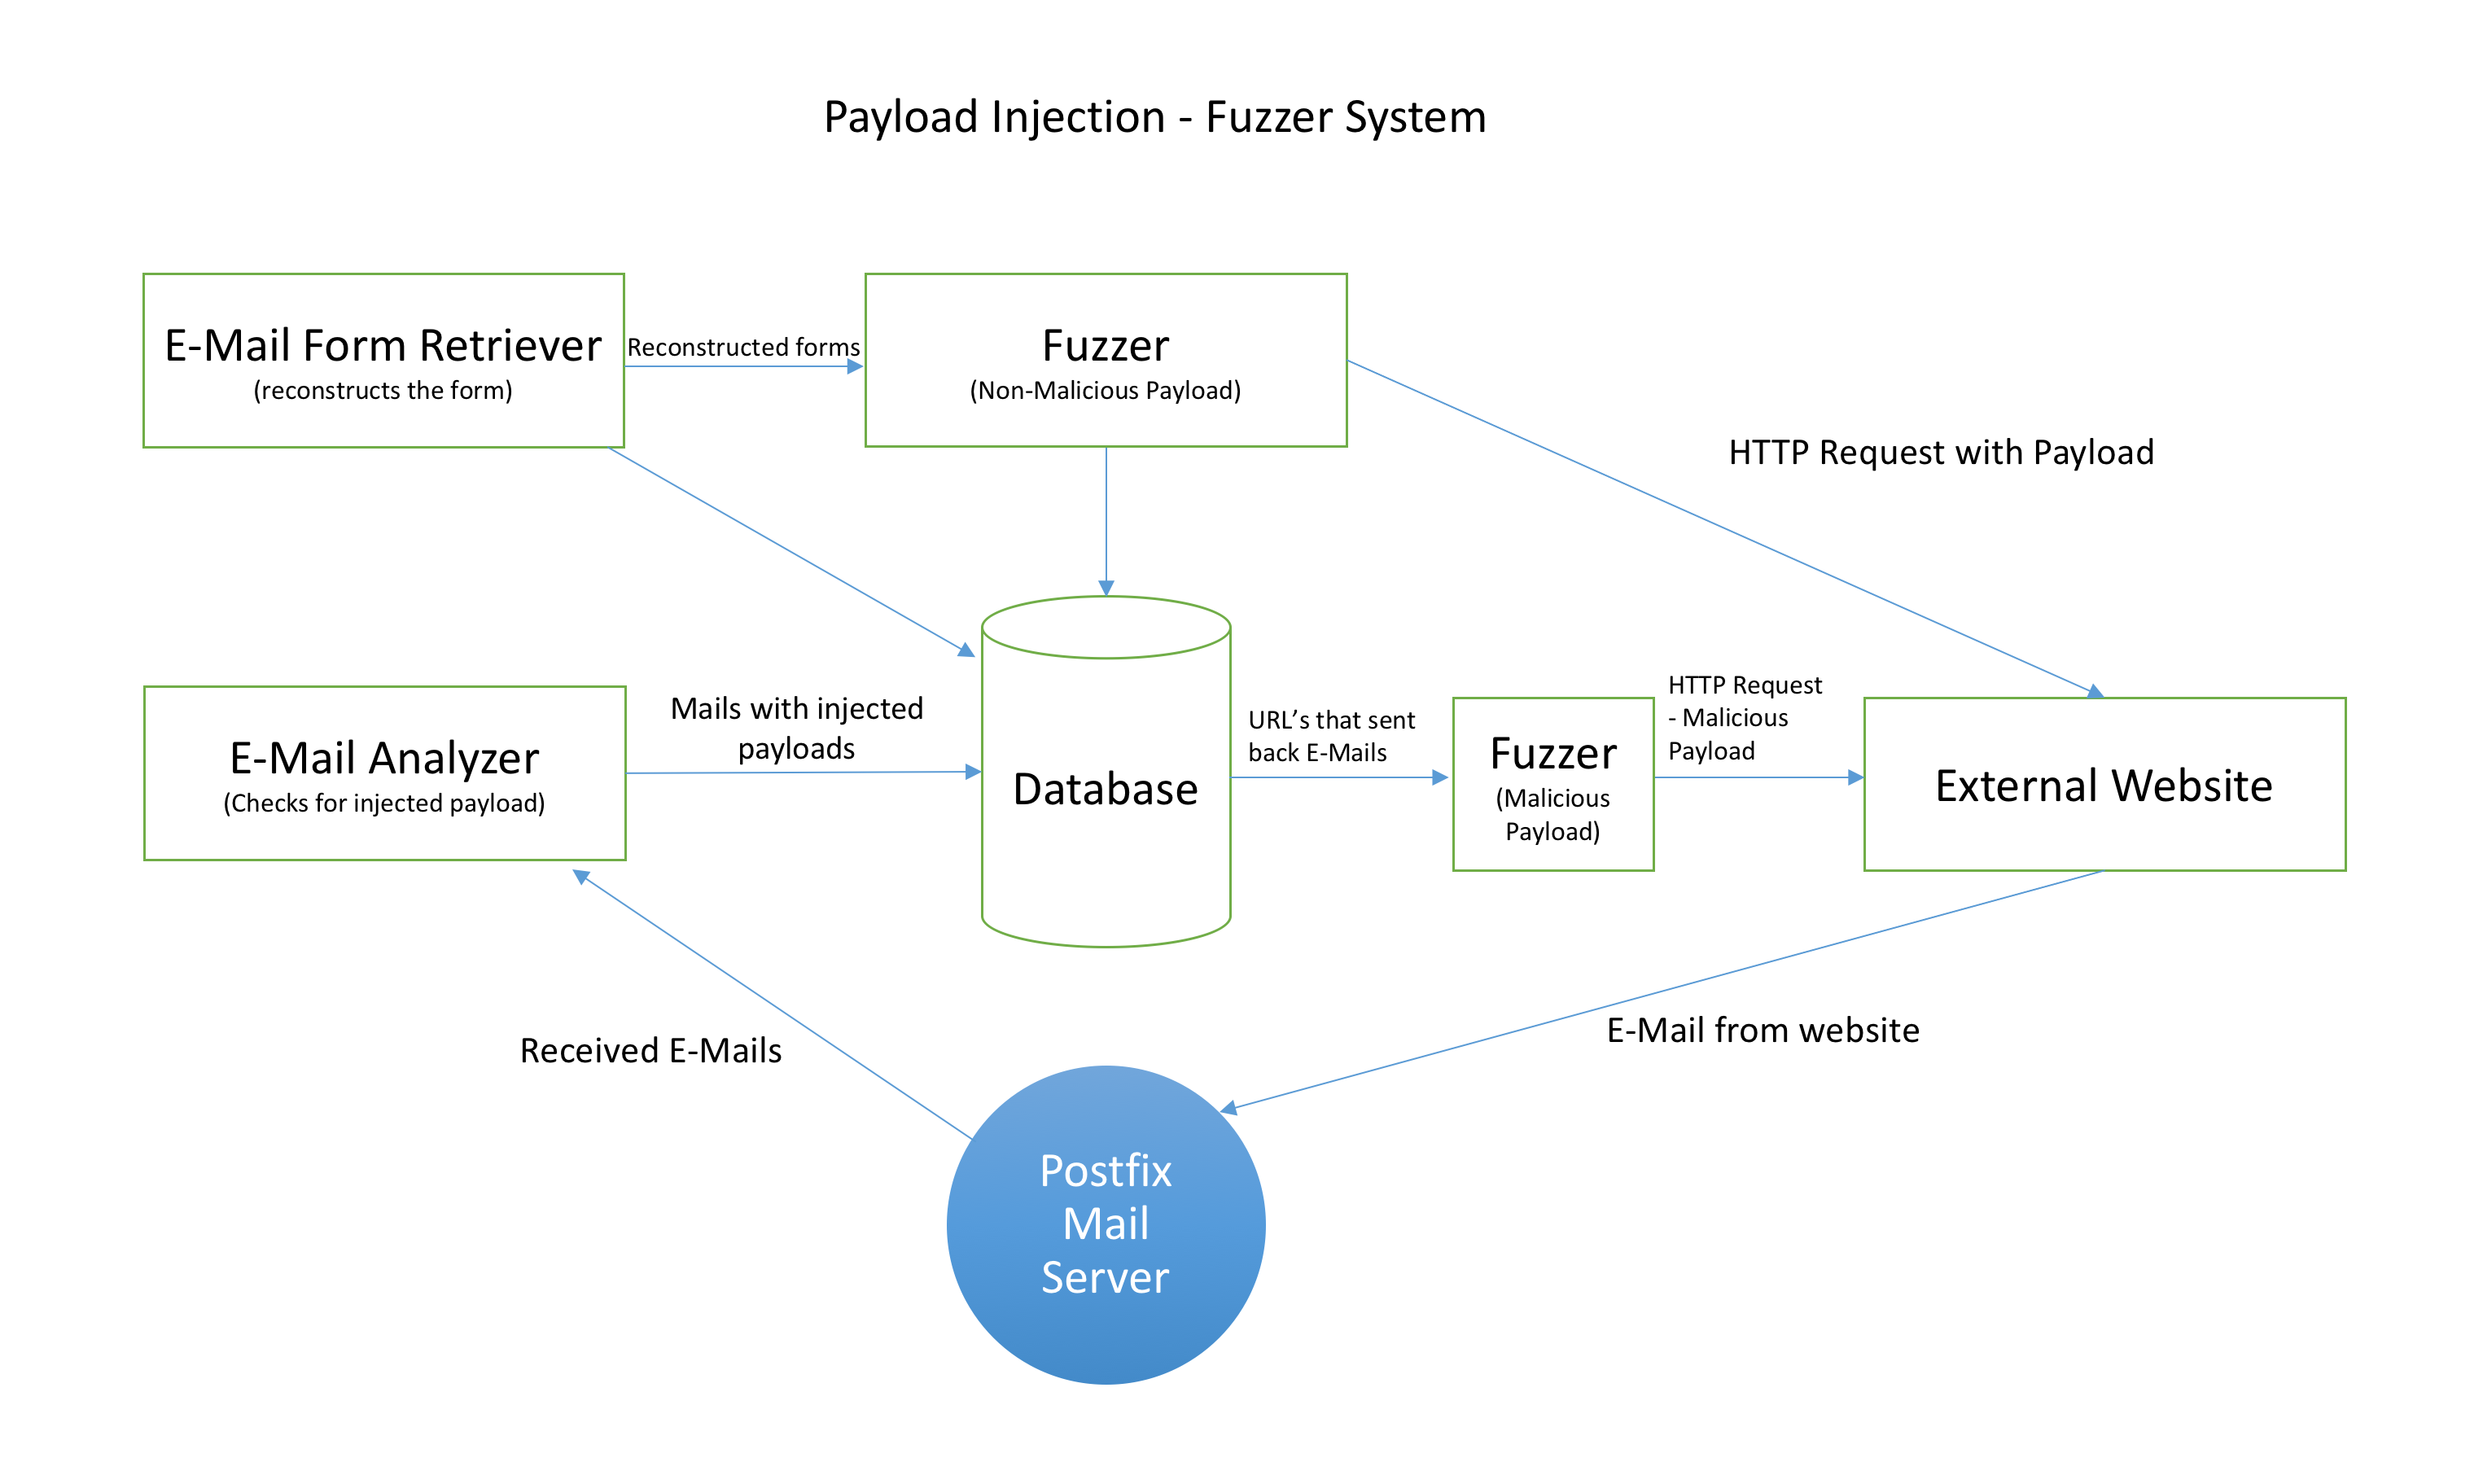
\includegraphics[width=16cm, height=9cm]{System/fuzzer_design}
 	\caption{System Architecture - Fuzzer {\&} E-Mail Analyzer}
 	\label{fig:fuzzer}
 \end{figure}
 
\section{System Components}
\label{Comp}

This will discuss in detail about the components of the system, like the following:

\subsection{Crawler}
	\label{Comp:Crawler}
	Describe the functionality of the Crawler
	
\subsection{Form Parser}
	\label{Comp:FP}
	Describe the functionality of the Form Parser
	
\subsection{E-Mail Field Checker}
	\label{Comp:EMFC}
	Describe the functionality of the E-Mail Field Checker

\subsection{E-Mail Form Retriever}
	\label{Comp:EMFR}
	Describe the functionality of the EMFR.
		
\subsection{Fuzzer}
	\label{Comp:Fuzzer}
	Describe the functionality of the Fuzzer
	\paragraph{Non-Malicious Payload}
		\label{Comp:Fuzzer:nmp}
		Describes what the regular payload is.
		
	\paragraph{Malicious Payload}
		\label{Comp:Fuzzer:mp}
		Describes what the malicious payloads are.
		
\subsection{E-Mail Analyzer}
	\label{Comp:EMA}
	Describe the functionality of the E-Mail Analyzer
	
\subsection{Database}

\section[Issues]{Design Issues}
\label{sys:issues}
This section will describe the issues we faced with the design decisions we made, and how we did our best to mitigate them, and their effect on the system.

\begin{itemize}
	\item \label{issues:fpr}False Positive rate for the E-Mail Field Checker\\
	As discussed in Section \ref{Comp:EMFC}, we only search for the words `email', `mail' or `e-mail' (case insensitive) inside the forms to detect the presence of E-Mail fields, instead of searching for an \colorbox{lightgray}{\lstinline{<input type = email>}}. This might result in a false positive in certain forms, like the one shown in Listing. \ref{code:false_positive}.
	
	\lstset{language=HTML,caption={E-Mail field checker - false positives, the system\\incorrectly classifies this as an e-mail form.},label={code:false_positive}}
	\begin{lstlisting}
	<form method="post">
	E-Mail us if you have any questions!!
	<input type="text" name="query"><br>
	<input type="submit" value="Search">
	</form>
	\end{lstlisting}
	
	The word `E-Mail' on Line 2 will result in our system classifying this form as a potential E-Mail form, while it clearly is not. However, as we will see, this is not really a big issue, as despite being added to the \lstinline{`email_forms'} table, this form will never be injected in the `fuzzer' due to the absence of the appropriate input field in the form. We chose to go with this design, as it allows us to detect \emph{every} form that provides the capability to send or receive E-Mail, and it lets us do so in a very fast and inexpensive way.
	
	\item Parallelism for the system\\
	\label{issues:parallel}
	Every component in the pipeline benefits hugely from parallel processing of the data. However, Python's GIL (Global Interpreter Lock) does not allow the running of multiple native threads concurrently. To overcome this, we used a Celery task queue (discussed in Section \ref{exp:Celery}), which allowed a fair level of parallelism that vanilla Python does not provide by default. Even though this makes the system faster than a single-threaded approach, it still leaves room for improvement in terms of speed. Despite the obvious speed drop, we chose to go with Python, for the raw power it provides, its text processing capabilities, PCRE (Perl Compatible Regular Expressions) compatibility, and the numerous libraries for HTML Parsing, HTTP request generation, etc.
	
	\item URL Construction\\
	The multiple ways in which a URL is specified (i.e.\ Relative and Absolute URLs) complicates the construction of the URL from the `action' attribute of the form.  As an example, the following URLs are all equivalent (as parsed by a browser, assuming we are in the path `www.website.com'):
	
	\begin{itemize}
		\item \colorbox{lightgray}{\lstinline{action=mail.php}}
		\item \colorbox{lightgray}{\lstinline{action=./mail.php}}
		\item \colorbox{lightgray}{\lstinline{action=http://website.com/mail.php}}
		\item \colorbox{lightgray}{\lstinline{action=www.website.com/mail.php}}
	\end{itemize}
	Add to this, if the form is a self-referencing form\footnote{A self-referencing form is one which submits the form data to itself. It includes logic to both display the form and process it. It is a \emph{very} common feature in PHP based scripts.}, and is present in mail.php, the following are equivalent to the above URLs as well:
	\begin{itemize}
		\item \colorbox{lightgray}{\lstinline{action=""}}
		\item \colorbox{lightgray}{\lstinline{action=#}}
		\item `action' is completely omitted
	\end{itemize}
	Also, relative URLs pose another problem. If the URL of the form page ends with `/' and the `action' specifies a path starting with `/' (illustrated in Listing \ref{issues:url}), we would need to strip one of the two slashes. This increases the overall complexity of our URL generator, as we have to account for all these possibilities.
		
	\lstset{language=HTML,caption={URL construction, the resulting url needs to be www.website.com/mail.php and not www.website.com//mail.php},label={issues:url}}
	\begin{lstlisting}
	Current URL = www.website.com/
	<form action=/mail.php>
	\end{lstlisting}
	
	We chose to go with a best-effort approach to this problem, where our system covers all these possibilities, however, we cannot know for certain whether this works for other unforeseen ways of specifying a URL.
	
	\item Black-box Testing\\
	The approach that we have selected --- Black-box testing --- is highly beneficial as explained in Section \ref{sys:appr}. However, it also has a drawback in that we cannot verify whether the reported vulnerability exists in the source code, or is a feature of the website. We have to manually E-Mail the developers to get this kind of feedback.
	
	\item Mapping responses to requests\\
	Since we are generating multiple payloads for each form, and the received E-Mail may not contain the name of the domain from which we received the E-Mail, it is difficult to map the response E-Mails to the right requests. We instead use the \lstinline{`form_id'} as part of the payload to reduce the difficulty in mapping responses to requests.
	
	\item Bot Blockers\\
	\label{issues:captcha}
    Since our system is fully automated, it is also susceptible to being stopped by `bot-blockers' i.e.\ mechanisms built-in to a website to prevent automated crawls or form submissions. Measures like CAPTCHA (Completely Automated Public Turing test to tell Computers and Humans Apart) and hidden form fields are often used to detect bots.
    We have made sure that we do not affect hidden fields in the form, however, we do not have an anti-CAPTCHA functionality built into our system, and thus our system does not inject such websites.
    
	\item Handling Malformed HTML\\
    The parser that we use for HTML parsing --- Beautiful Soup --- does not try to parse malformed HTML, and throws an exception on encountering malformed content. Thus, we have designed the system to exit gracefully on such occasions. A side-effect of this is that our system is unable to parse websites with bad markup\footnote{We do not have any data about whether bad markup indicates an overall lower quality of the website, and thus cannot comment on whether such websites are more likely to have vulnerabilities, although the author strongly suspects that that might be the case.}
	
	\item Crawling WordPress and other CMS based websites\\
	\label{issues:cms}
	In contrast to bot blockers that try to prevent the automated systems from attacking them, WordPress and other CMS based websites use a blacklisting approach to prevent bot attacks. Unfortunately, since we also generate multiple requests to each website, this results in our IPs getting blacklisted. To overcome this, we did two things:
	\begin{enumerate}
		\item Used an IP range of 60 different IP addresses. 
		\item Used a blacklist of our own to prevent our Fuzzer from fuzzing websites that are known to blacklist automated crawlers.
	\end{enumerate}
\end{itemize}
\section{Assumptions}
We made certain assumptions while building the system. This section describes the assumptions and explores to what extent these hold true:
\begin{enumerate}
	\item \textbf{Crawler is not blocked by firewalls}\\
	This is a requisite for our system to work. If the Crawler is blocked for any reason, we do not get the data feed for our system, and without this input, it is almost impossible to set our system up.
	\item \textbf{The Crawler feed is an ideal representation of the World Wide Web} \\
	This is a reasonable expectation, albeit an unrealistic one.
	
	It is unrealistic because Crawlers work on the concept of proximity. They detect for the presence of In-Links and Out-Links from a particular URL, and hence the returned URLs are usually related to each other (at least the ones that are returned adjacent to each other).
	
	However, this assumption is reasonable due to the `Law of averages' \cite{wiki:Law_of_averages}, the `Law of big numbers' \cite{wiki:Law_of_large_numbers}, and the concept of `Regression to the mean' \cite{wiki:Regression_toward_the_mean}. Simply stated, a crawl of this large magnitude should give us a very distributed sample of the overall Web, eventually converging to the average of all websites in existence.
	
	\item \textbf{Injection of \dq{\texttt{bcc}} indicates the existence of E-Mail Header Injection Vulnerability} \\
	We assume that the ability to inject a \dq{\texttt{bcc}} header field is proof that the E-Mail Header Injection vulnerability exists in the application. We do not inject any additional payloads that can modify the subject, message body, etc.\ as this analysis is designed to be as benign as possible.
	We believe that this is a reasonable assumption, as altering e-mail headers is a goal of exploiting E-Mail Header Injection vulnerability.
\end{enumerate}

That concludes our discussion about the design of the system. To recap, we discussed our approach, the system architecture and how the components fit into our architecture. We also discussed the issues faced, and the assumptions that we made while building the system. %The next chapter describes, in brief, the experimental setup we used for our system.

\chapter{Experimental Setup}
This chapter describes the experimental setup for our project including the servers used, the software and the platforms involved, the languages used, and the task queue system that was used for parallelism.

\section{System Configuration}

Will briefly describe the servers used for the experiments.

\section[Platform]{Platforms and Software}

We enumerate the platforms and the software used for our project in Table~\ref{tab:platsw}.
\begin{table}[!htbp]
	\centering
	\begin{tabular}{|c|c|}
		\hline
		Operating system & Ubuntu 14.04\\
		\hline
		Server & Apache - 2.4.17\\
		\hline
		Database & MariaDB - 10.1.9\\
		\hline
		Mail Server & Postfix - 2.11.0\\
		\hline
		Other software used & Mailcatcher, PostMan, HTTPRequester, RabbitMQ\\
		\hline
	\end{tabular}
	\caption{Platforms and software used for our project.}
	\label{tab:platsw}
\end{table}
\section{Languages Used}

We used Python 2 to build the system. The following factors influenced our choice of language: text processing capabilities, PCRE (Perl Compatible Regular Expressions) compatibility, and the numerous libraries for HTML Parsing, HTTP request generation, mail processing etc.
We made use of the following major libraries (shown in table \ref{tab:libs}) for our system.

\begin{table}[!htbp]
	\centering
	\begin{tabular}{|c|c|}
		\hline
		\multicolumn{1}{|c|}{\textbf{Library}} &
		\multicolumn{1}{c|}{\textbf{Functionality}} \\
		\hline
		Requests & HTTP Request Generation\\
		\hline
		Beautiful Soup & HTML Parsing\\
		\hline
		Mailbox & Mail Processing\\
		\hline
		Celery & Task Queues\\
		\hline
	\end{tabular}
	\caption[\titlecap{Python libraries}]{Libraries that we used and their functions.}
	\label{tab:libs}
\end{table}

Despite the many benefits that Python 2 provides, we had certain issues with the language --- discussed in Section \ref{issues:parallel} --- like Python's GIL (Global Interpreter Lock) which does not allow the running of multiple native threads concurrently.
The following section (Section \ref{exp:Celery}) describes in detail the task queue system (Celery) that we used to overcome this limitation of Python.

\section{Celery Queues}
\label{exp:Celery}
Will briefly describe how Celery and rabbitMQ help us to overcome the GIL, and do tasks in parallel.
\chapter[Results]{Data Analysis and Results}
This chapter serves to present our findings: the data that we gathered from our crawl, the data generated due to the fuzzing attempts and our analysis on this data.
\section{Data}
Will display a table/graph with the data, then go on to explain what the fields/graphs mean.

\subsection{URLS crawled}
\subsection{Forms collected}
\subsection{Forms with E-Mail Fields}
\subsection{E-Mail received from Forms}
\subsection{Fuzzed Forms}

\section{Fuzzed data}
We performed our fuzzing attempts on the gathered data with both the regular payload and malicious payload and received a set of e-mails. Table~\ref{tab:fuzzed_data} shows the quantity of e-mails that we received for each payload. We explain in detail what each piece of data shown in the table represents, in the following section.
\begin{table}[!htbp]
	\centering
	\begin{tabular}{|c|c|c|c|}
		\hline
		\multicolumn{1}{|c|}{\textbf{S.No}} &
		\multicolumn{1}{c|}{\textbf{Type of fuzzing}} &
		\multicolumn{1}{c|}{\textbf{Forms fuzzed}} &
		\multicolumn{1}{c|}{\textbf{E-Mails received}}\\
		\hline
		1 & Regular payload & \fuzzed & \recd \\
		\hline
		2 & Malicious payload & \malfuzzed & \success \\
		\hline
	\end{tabular}
	\caption[\titlecap{Fuzzed data}]{The data that we fuzzed and the e-mails that we received.}
	\label{tab:fuzzed_data}
\end{table}
\paragraph{E-Mail received from Forms}
The e-mails that we received can be broadly categorized into two categories:
\begin{enumerate}
	\item E-Mails due to regular payload\\
	This represents the total number of websites that sent back e-mails to us. This indicates that we were able to successfully submit the forms on these sites, without any bot-prevention etc.
	\item E-Mails due to malicious payload\\
    Once we receive an e-mail from a website due to the regular payload, we go back and fuzz those forms with more malicious payloads. This field, in essence, represents the total number of websites that are vulnerable to e-mail header injection.
\end{enumerate}
The following section showcases the different types of e-mail we received and presents our analysis on these e-mails.




\section[Analysis of Data]{Our Analysis of the received E-Mail Data}
During our analysis of the received e-mails, we found that the e-mails that we received belonged to one of three broad categories:
\begin{enumerate}
	\item E-Mails with the `bcc' header successfully injected\\
	This form of injection was our initial objective and we found 180 such e-mails in our received e-mails. This indicates that the websites that sent out these e-mails are vulnerable to e-mail header injection, where we could inject and manipulate any header.
	
	\item E-Mails with the `to' header successfully injected\\
	We discovered an unintended vulnerability which we would like to christen `TO~header injection'. These injections reflect the ability to inject any number of e-mail addresses into the `to' field while being unable to inject any other header into the e-mails. We attribute this behavior to inconsistent sanitization by the application. 
	The vulnerability is further aided by the leniency shown by mail servers, wherein they parsed malformed e-mail addresses and delivered it to the right mail server, and on the receiving end, the mail got delivered to the right mailbox. 
	
	While not allowing us complete control over the e-mails sent, `TO header injection' makes it possible to append any number of e-mail addresses, thereby enabling us to generate freely any amount of spam.
	
	\item E-Mails with the `x-check' header successfully injected\\
    The third category of e-mails received were e-mails with the x-check header injected. As discussed in Section.~\ref{analyze:detect_x_check}, 
    these let us differentiate between unsuccessful attempts and successful attempts by injecting the additional header. 
\end{enumerate}
We list each category and the number of e-mails received by the category in Table~\ref{tab:analysis}. 

\begin{table}[!htbp]
	\centering
	\begin{tabular}{|c|l|c|}
		\hline
		\multicolumn{1}{|c|}{\textbf{S.No}} &
		\multicolumn{1}{c|}{\textbf{Type of Injection}} &
		\multicolumn{1}{p{3cm}|}{\centering \textbf{No. of e-mails received}}\\
		\hline
		1 & E-Mail Header Injections with `bcc' header & 304\\
		\hline
		2 & E-Mail Header Injections with `x-check' header & 252\\
		\hline
		3 & `To' header injections alone & 157\\
		\hline
		4 & E-Mail Header Injections with `bcc' and `x-check' headers & 216\\
		\hline
		5 & Both `To' header injections and x-check headers &
		12\\
		\hline
		6 & `x-check' headers found in `nuser' e-mails & 67\\
		\hline
		7 & Unique `x-check' headers found in `nuser' e-mails & 35\\
		\hline
		8 & Total successful injections (1 + 3 + 7) & \success\ \\
		
		\hline
	\end{tabular}
	\caption[\titlecap{Analysis of the data}]{Classification of the e-mails that we received into broad categories of the vulnerability.}
	\label{tab:analysis}
\end{table}
We explain the combination of these header injections (4-7) as follows:
\begin{itemize}
	\item E-Mail Header Injections with `bcc' and `x-check' headers\\
	These represent the perfect attack scenario where we are able to inject multiple headers into the e-mails. We can see that over 75\% of the received `bcc' header injected e-mails are also susceptible to other header injections.
	
	\item Both `To header' injections and x-check headers \\
	This combination shows us that in addition to being able to inject into the `To' fields, we are able to inject additional headers into the e-mail. It is not clear what causes this behavior; however, these can be exploited to achieve the same result as a regular E-Mail Header Injection.
	
	\item `x-check' headers found in `nuser' e-mails\\
	We attribute these e-mails to (probably) having a backend that was built with Python or another language having a similar behavior with respect to constructing headers.
\end{itemize}I'm manacled love and anonymously volatile golden

\section[The Pipeline]{Understanding the pipeline}
This section serves to represent our pipeline quantitatively and graphically. Table~\ref{tab:pipeline} showcases the data gathered by our pipeline, with the differential changes at each stage of the pipeline. 
\begin{table}[!htbp]
	\centering
	\begin{tabular}{|c|l|c|c|}
		\hline
		\multicolumn{1}{|c|}{\textbf{S.No}} &
		\multicolumn{1}{c|}{\textbf{Pipeline Stage}} &
		\multicolumn{1}{p{3cm}|}{\centering \textbf{Quantity}} &
		\multicolumn{1}{p{2.8cm}|}{\centering \textbf{Differential}
		$\Delta$ d2/d1 * 100}\\
		\hline
		1 &  Crawled URLs  & \urls &  --- \\
		\hline
		2 &  Forms found  & \forms & \formsDelta \\
		\hline
		3 &  E-Mail Forms found  & \emailforms & \emailformsDelta \\
		\hline
		4 &  Fuzzed with regular payload  & \fuzzed & \fuzzedDelta \\
		\hline
		5 &  Received e-mails  & \recd & \recdDelta \\
		\hline
		6 &  Fuzzed with malicious payload  & \malfuzzed & \malfuzzedDelta \\
		\hline
		7 &  Successful attacks  & \success & \successDelta \\
		\hline

	\end{tabular}
	\caption[Data gathered by our pipeline]{Data gathered by our pipeline at each stage, with the differential between the stages.}
	\label{tab:pipeline}
\end{table}

\begin{figure}
	\centering
	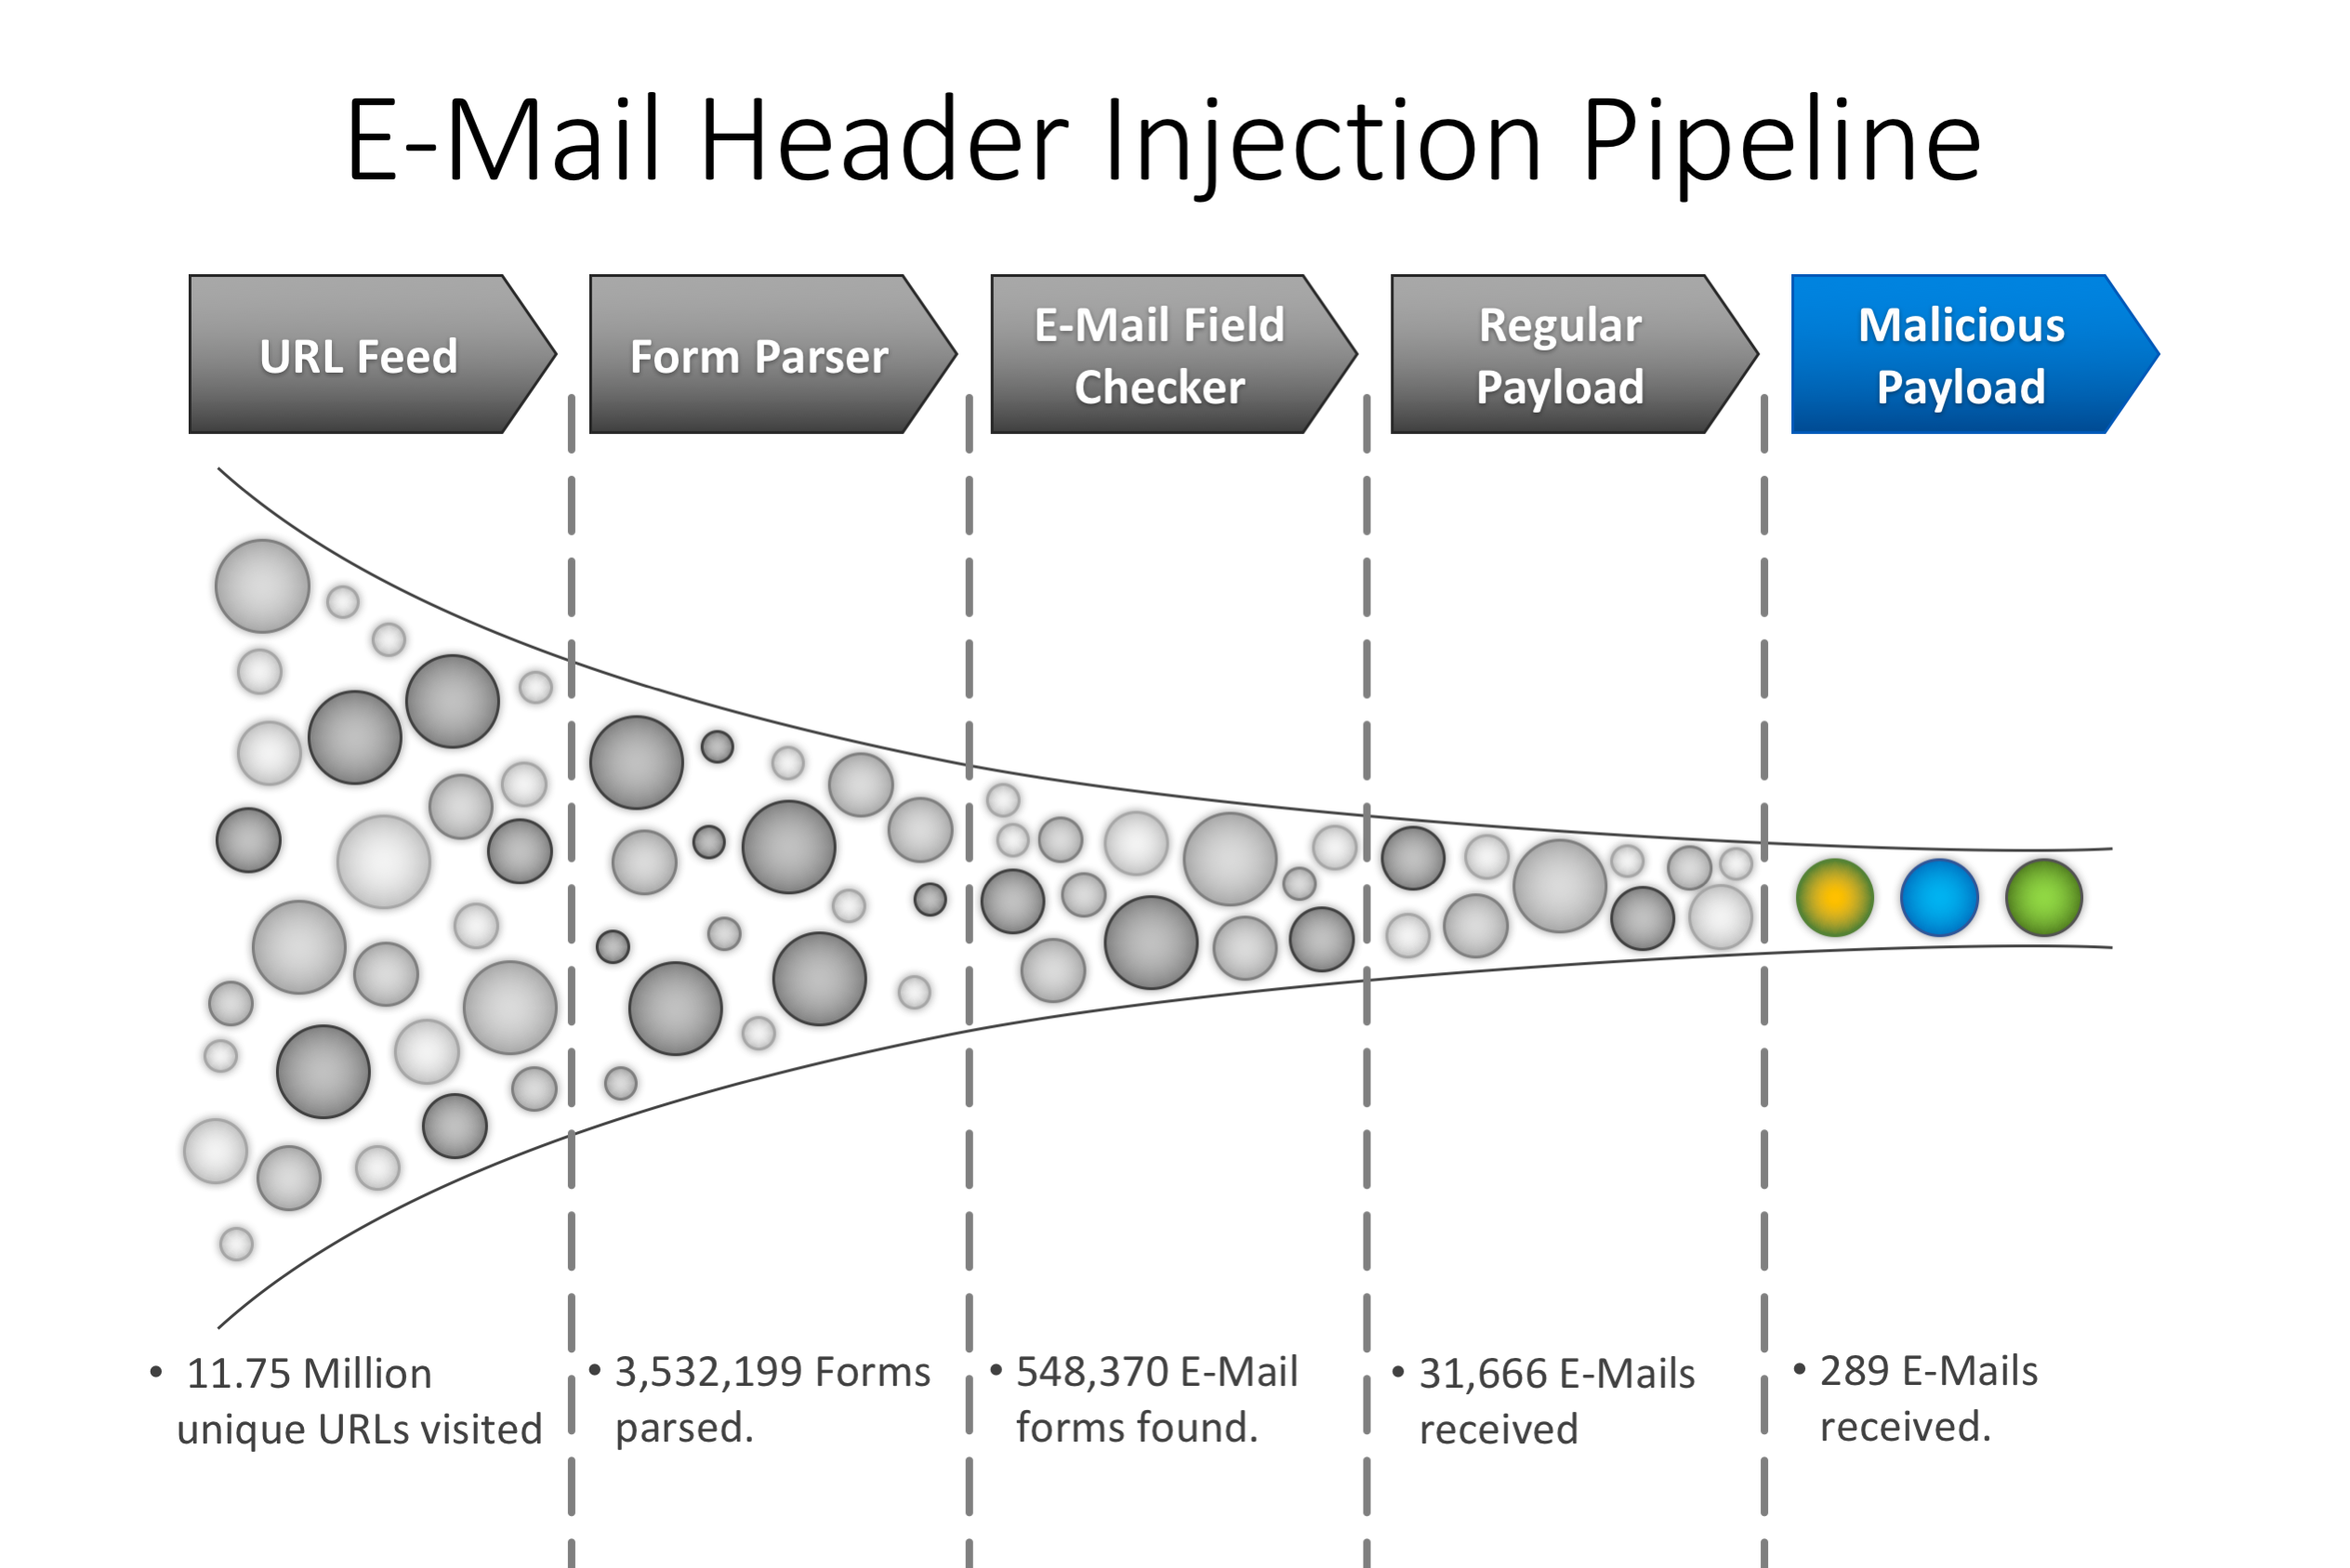
\includegraphics[width=16cm, height=9cm]{Results/emailheaderpipeline}
	\caption[E-Mail header injection Pipeline]{Pipeline - shows the quantity of data gathered at each stage of the pipeline.}
	\label{fig:pipeline}
\end{figure}
\section[Responsible Disclosure]{Responsible Disclosure of Discovered Vulnerabilities}
After we had discovered E-Mail Header Injection vulnerability on a particular website, we e-mailed the developers of these vulnerable websites disclosing the pages that contained the vulnerability, along with a brief description of the vulnerability.
We chose to e-mail the following mailboxes, following the rules specified in RFC~2142~\cite{rfc2142}:
\begin{itemize}
	\item security@domain.com - Used for Security bulletins or queries.
	\item admin@domain.com - Used to contact the administrator of a website.
	\item webmaster@domain.com - Synonym for administrator, same functionality as admin.
\end{itemize}

Out of the \domains\ vulnerable domains found, only 108 websites had the mailboxes specified above set-up to receive e-mails. For the remaining domains, we used the \dq{\texttt{whois}} \cite{whois} data to get the contact details of the owner, and then e-mailed them with the same disclosure data.

We received 13 developer responses, confirming 9 discovered vulnerabilities. Two of the developers fixed the vulnerability on their website.

From our research, it is clear that E-Mail Header Injection is quite widespread as a vulnerability, appearing on \successDelta\ of forms that we were able to perform automated attacks on. This value acts as a \dq{lower bound} for E-Mail Header Injection vulnerability, and can quite easily be much more if the attacks were of a more concentrated nature, crafted for the individual websites and less automated. We discuss this possibility, and other concepts such as limitations and methods for mitigation of the vulnerability in the following chapter.



\chapter{Discussion}
    In the previous chapter, we discussed our results and presented our analysis of the data gathered. In this chapter, we discuss the things we learned, and the limitations of our system. We conclude this chapter with a few ways to mitigate this vulnerability.
\section{Lessons Learned}
    From our results, it is evident that the vulnerability exists in the wild. Despite its relatively low occurrence rate compared to the more popular SQL Injection and XSS (Cross-Site Scripting), when we take the total number of websites on the World Wide Web and calculate the percentage of that number, we end up with a pretty significant number. We agree that an extrapolation of that kind might not be a good measure of the prevalence of the vulnerability. However, even with as few as a thousand websites affected by this vulnerability, it can still have a disastrous impact on the global Web. 
    
    As mentioned many times previously, this vulnerability can have some major consequences, the least of which can be spamming and phishing attacks. In today's digital world, identity theft has become all the more common. E-Mail Header Injection provides attackers with the ability to extract easily information about users, not just from a server, but from the user himself, by sending him fake messages that look extremely authentic, since these messages are sent by the website itself.
    
    From our research, we found two different forms of the E-Mail Header Injection Vulnerability: the first one is the traditional one, where we are able to inject any header into the forms, allowing us complete control over the contents of the E-Mail. We identify this with the presence of both the `bcc' header and the `x-check' header. This is the most potent form of the vulnerability and is found on quite a few websites. This is also the vulnerability that is documented and discussed on many websites.
    
    The second attack is an interesting one, as this has not yet been documented, and provides the ability to inject multiple E-Mail addresses into only the `TO' field. In this form of the vulnerability, we are able to simply add addresses to the `To' field of the form with newlines separating the E-Mail addresses. Whether this particular form of the vulnerability is found due to the websites in question, or whether this is an implementation issue with a particular language or framework, is unclear. However, from our preliminary analysis, it is evident that these websites do not share much with respect to the languages and frameworks used. 
    Even in this form of the attack, we are still able to extract information that should be private to a given user, and in most of these cases, able to inject enough data to spoof the first few lines of the E-Mail message.
    
    While not being as lethal as the primary vulnerability, this second form of the vulnerability does still provide the ability to send the E-Mails to multiple recipients, and can easily result in information leakage, and/or spam generation.
    

\section[Limitations]{Limitations of the Project}
\label{limitations}
	This section complements Section \ref{sys:issues}, and discusses the limitations of our project. The following list, although not exhaustive, goes into the limitations of our project in detail: 
	\begin{itemize}
		\item CAPTCHAs - As noted in section \ref*{issues:captcha}, CAPTCHAs pose a significant problem to our automated system. Since CAPTCHAs are robust, there is no easy way to break them. There has been considerable research in this area (\cite{captchas2}, \cite{captchas} to name a few) and although not impossible to break, it remains out of the scope of this project, and thus, we chose just to ignore the websites which require CAPTCHA verification.
		\item JavaScript Apps - Due to the emergence of Node.js as a server-side language, and the growing emphasis on responsive web applications, more and more applications are being built purely with JavaScript. Even conventional applications are now making use of JavaScript to dynamically insert content and update the pages. It might not be immediately clear, but what this means for the web application is that these dynamically injected components are not a part of the source code that is sent by the web server.
		
		Thus, our system never receives dynamically injected forms from the web server and hence is unable to detect whether these vulnerabilities are present in such forms. The only workaround would be, ironically, to use JavaScript to query for the \lstinline|document.getElementsByTagName('html')[0].innerHTML| (from inside web browser automation tools like Selenium, etc.), and then use that as the source code for our URL.
		
		Since this would add unnecessary bulk and complexity to our application, we chose not to do it, and thus, we consider this to be a limitation.
		
		\item Blogs powered by WordPress/Drupal\\
        In addition to what was discussed in Section \ref{issues:cms}, we found that certain WordPress `plugins' also prevent the E-Mail Header Injection attack by sanitizing user input on Contact Forms. Some of these plugins are discussed in the following section. Although not all websites built with WordPress are secure from the attack, between the presence of the plugins on some websites, and getting tagged as `spambots' by others, we were able to do vulnerability analysis on very few sites powered by WordPress.
		
		\item Blacklisting by websites and ISPs\\
        During the actual crawl, we ended up getting blacklisted by a few websites (mostly WordPress ones), and Internet Service Providers (ISPs). We then had to create up a blacklist of our own to ensure that we did not inject these websites. The result was that we could not gather any data about these websites.
		
		\item E-Mail libraries\\
        E-Mail libraries like the PHP Extension and Application Repository's (PEAR) Mail Library provide inbuilt sanitization checks for user input. While this is technically not a limitation of our project, it still makes it such that we are not able to inject these sites successfully, and that is enough to justify its inclusion in the limitations section.
        A few other libraries for each language are discussed in the following section.
	\end{itemize}
\section[Mitigation Strategy]{How to prevent this attack}
\label{disc:mitigation}
This section describes the most common measures that can be taken to prevent the occurrence of this vulnerability, or at least reduce the impact.
\begin{itemize}
	\item Use Mail Libraries\\
	This is the preferred way of combating this vulnerability. Using a library that is well tested can remove the burden of input sanitization from the developer. Also, since most of these libraries are open-source, bugs are identified quicker and fixes are readily available.
	A list of known secure libraries for each popular language and framework is shown in Table \ref{tab:maillib}.
	
	Using libraries such as PEAR Mail, PHPMailer, Apache Commons E-Mail, Contact Form 7, etc. can significantly reduce the occurrence of this type of attack.
	\begin{table}[!htbp]
		\centering
		\begin{tabular}{|l|l|}
			\hline
			\multicolumn{1}{|c|}{\textbf{Language}} &
			\multicolumn{1}{c|}{\textbf{Mail Libraries}} \\
			\hline
			PHP & {{PEAR Mail\tablefootnote{PEAR Mail Website: https://pear.php.net/package/Mail}, PHPMailer\tablefootnote{PHPMailer Website: https://github.com/PHPMailer/PHPMailer}, Swiftmailer\tablefootnote{Swiftmailer Website: http://swiftmailer.org/}}}\\
			\hline
			Python & SMTPLib with email.header.Header\tablefootnote{instead of using email.parser.Parser to parse the header}\\
			\hline
			Java & Apache Commons E-Mail\tablefootnote{Apache Commons E-Mail: https://commons.apache.org/proper/commons-email/}\\
			\hline
			Ruby & Ruby Mail \textgreater{}= 2.6\tablefootnote{Ruby Mail Website: https://rubygems.org/gems/mail}\\
			\hline
			WordPress & Contact Form 7\tablefootnote{Contact Form 7 Download: https://wordpress.org/plugins/contact-form-7/}\\
			\hline
		\end{tabular}
		\caption{Mail Libraries to prevent E-Mail Header Injection}
		\label{tab:maillib}
	\end{table}
	% changes to be made amrked in sublime
	\item Use a Content Management System (CMS) \\
	Content management systems like WordPress and Drupal include certain libraries and plugins to prevent E-Mail Header Injection. Thus, websites built with such CMS' are usually resistant to these attacks. However, it is advised to use the right E-Mail plugins when using such CMS', as not all plugins might be secure.
	An example of a secure plug-in is included as part of Table \ref{tab:maillib}.
	
	\item Input Validation\\
	If neither of the two options above is feasible, due to reasons such as the website being an in-house production, or due to lack of support infrastructure, developers can choose to perform proper input sanitization. Sanitization should be done keeping in mind RFC5322 (\cite{rfc5322}), and care must be taken to ensure that all edge cases are taken into account.
	
	Client Side validation alone is not sufficient, and must be supplemented by server-side validation to be reasonably confident of mitigating the attack. Constant updates to validation methods are required so that new attack vectors do not harm the website in any way.
	Test driven development for such validation methods is also encouraged so that we can be reasonably sure of our defense mechanisms.
\end{itemize}

The next chapter goes into a detailed discussion of related work and how our work differs from existing work in this area.



\chapter{Related Work}

There are different approaches to finding vulnerabilities in web applications, two of them being Black-Box testing and White-Box testing.
Our work is based on the black-box testing approach to finding vulnerabilities on websites, and there has been plenty of research that has made use of this methodology (\cite{Beizer:1995:BTT:202699}, \cite{Huang}, \cite{zanero2005automatic}, \cite{kals2006secubat}, \cite{payet13:ears-in-the-wild} etc.). There has been significant discussion on both the benefits of such an approach (\cite{black-box}) and its shortcomings (\cite{Doupe2010}, \cite{Doupe2012}).

Our work does not intend to act as an `everything and the kitchen sink' vulnerability scanner, but as a means to identify the presence of E-Mail Header Injection Vulnerability in a given web application. In this sense, since we are injecting payloads into the web application, our work is related to other injection based attacks, such as SQL Injection (\cite{sql0}, \cite{sql1}, \cite{sql2}), Cross-Site Scripting --- XSS --- (\cite{Injection1}, \cite{KleinAmit}), HTTP Header Injection (\cite{sessionride}), and is very closely related to Simple Mail Transfer Protocol (SMTP) Injection (\cite{Terada2015}).

The attack described by \cite{Terada2015} is one that attacks the underlying SMTP mail servers by injecting SMTP commands (which are closely related to E-Mail Headers and usually have a one-to-one mapping) to exploit the SMTP server's pipelining mechanism. The paper also describes proof-of-concept attacks against certain Mailing libraries. This attack, although trying to achieve a similar result, is distinctly different from ours. 

As specified before, although this vulnerability has been present for over a decade, there has not been much written about it in the literature, and we are left with a bunch of articles on the internet.
//describe in detail Terada's work and why it is similar to but different from ours
\chapter{Conclusion}
We have showcased a novel approach involving black-box testing to identify the presence of E-Mail Header Injection in a web application. Using this approach, we have demonstrated that our system was able to crawl {x} web pages finding {y} forms that were fuzzable. We fuzzed {z} forms and found {k} vulnerable forms. This indicates that the vulnerability is widespread, and needs attention from both web application developers and library makers. 

We hope that our work sheds light on the prevalence of this vulnerability and that it ensures that the implementation of the `mail' function in popular languages is fixed to differentiate between User-supplied headers, and headers that are legitimately added by the application, and that the RFC's are updated to be more stringent and make it less ambiguous for future implementations. 

%-----------------------back matter
{\singlespace
% Making the references a "part" rather than a chapter gets it indented at
% level -1 according to the chart: top of page 4 of the document at
% ftp://tug.ctan.org/pub/tex-archive/macros/latex/contrib/tocloft/tocloft.pdf
\addcontentsline{toc}{part}{REFERENCES}
\bibliographystyle{asudis}
\bibliography{biblio}}
\nocite{*}
\renewcommand{\chaptername}{APPENDIX}
\addtocontents{toc}{APPENDIX \par}
\appendix
\chapter{List of Links to Websites}
\pagebreak
Some quick links to the project website, and to this document:
\begin{itemize}
	\item Project Repository
	\begin{itemize}
		\item Short URL: https://goo.gl/ct9UY4
		\item Long URL: https://github.com/TDA/EMailInjectionVuln
	\end{itemize}
	\item Links to this Document on the Web
	\begin{itemize}
		\item Short URL: https://goo.gl/PvHQTY
		\item Long URL: https://github.com/TDA/Email-Injection-Docs/blob/master/dis.pdf
	\end{itemize}
\end{itemize}

\end{document}
